\section{Aprendizaje Automático}

\begin{frame}
    \frametitle{Aprendizaje Automático}

    \begin{itemize}
        \item Objetivo: hacer aprender a una computadora
        \item En la \emph{clasificación} se intenta aprender la categoría de una entidad.
    \end{itemize}
\end{frame}

\subsection{Clasificadores}
\begin{frame}
    \frametitle{Clasificadores}
    
    \begin{itemize}
        \item Un clasificador decide en base a \emph{características} y a ciertas suposiciones.
    \end{itemize}
\end{frame}

\begin{frame}
    \frametitle{Support Vector Machine (SVM)}

    \begin{center}
        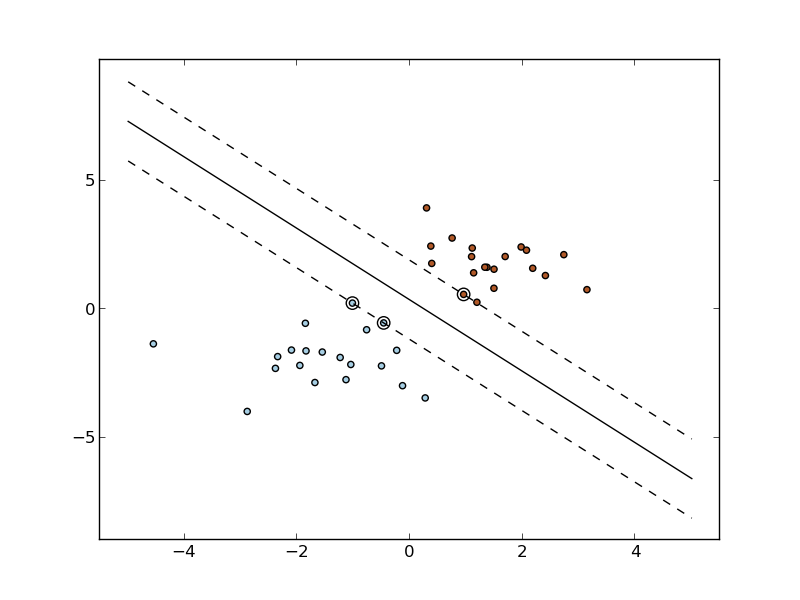
\includegraphics{svm.png}
    \end{center}
\end{frame}

\begin{frame}
    \frametitle{Árbol de decisión}

    \begin{center}
        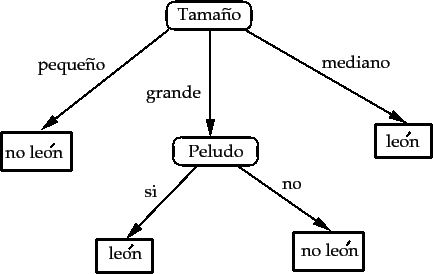
\includegraphics{dts.png}
    \end{center}
\end{frame}

\begin{frame}
    \frametitle{Sobreajuste}

    \begin{center}
        \includesvg[height=7cm, svgpath = imagenes/]{overfitting}
    \end{center}
\end{frame}

\begin{frame}
    \frametitle{Naïve Bayes}

    \begin{center}
        \[
            P(A|B) = \frac{P(B|A) P(A)}{P(B)}
        \]

        \begin{align*}
            c &= \argmax_{c \in C} P(c|a_1, \ldots, a_n) \\
            &= \argmax_{c \in C} \frac{P(a_1, \ldots, a_n|c) P(c)}{P(a_1, \ldots, a_n)} \\
            &= \argmax_{c \in C} P(a_1, \ldots, a_n|c) P(c) \\
            &\approx \argmax_{c \in C} P(c) \prod_{i=1}^n P(a_i|c) \\
        \end{align*}
    \end{center}
\end{frame}

\begin{frame}
    \frametitle{k Nearest Neighbors (kNN)}

    \begin{center}
        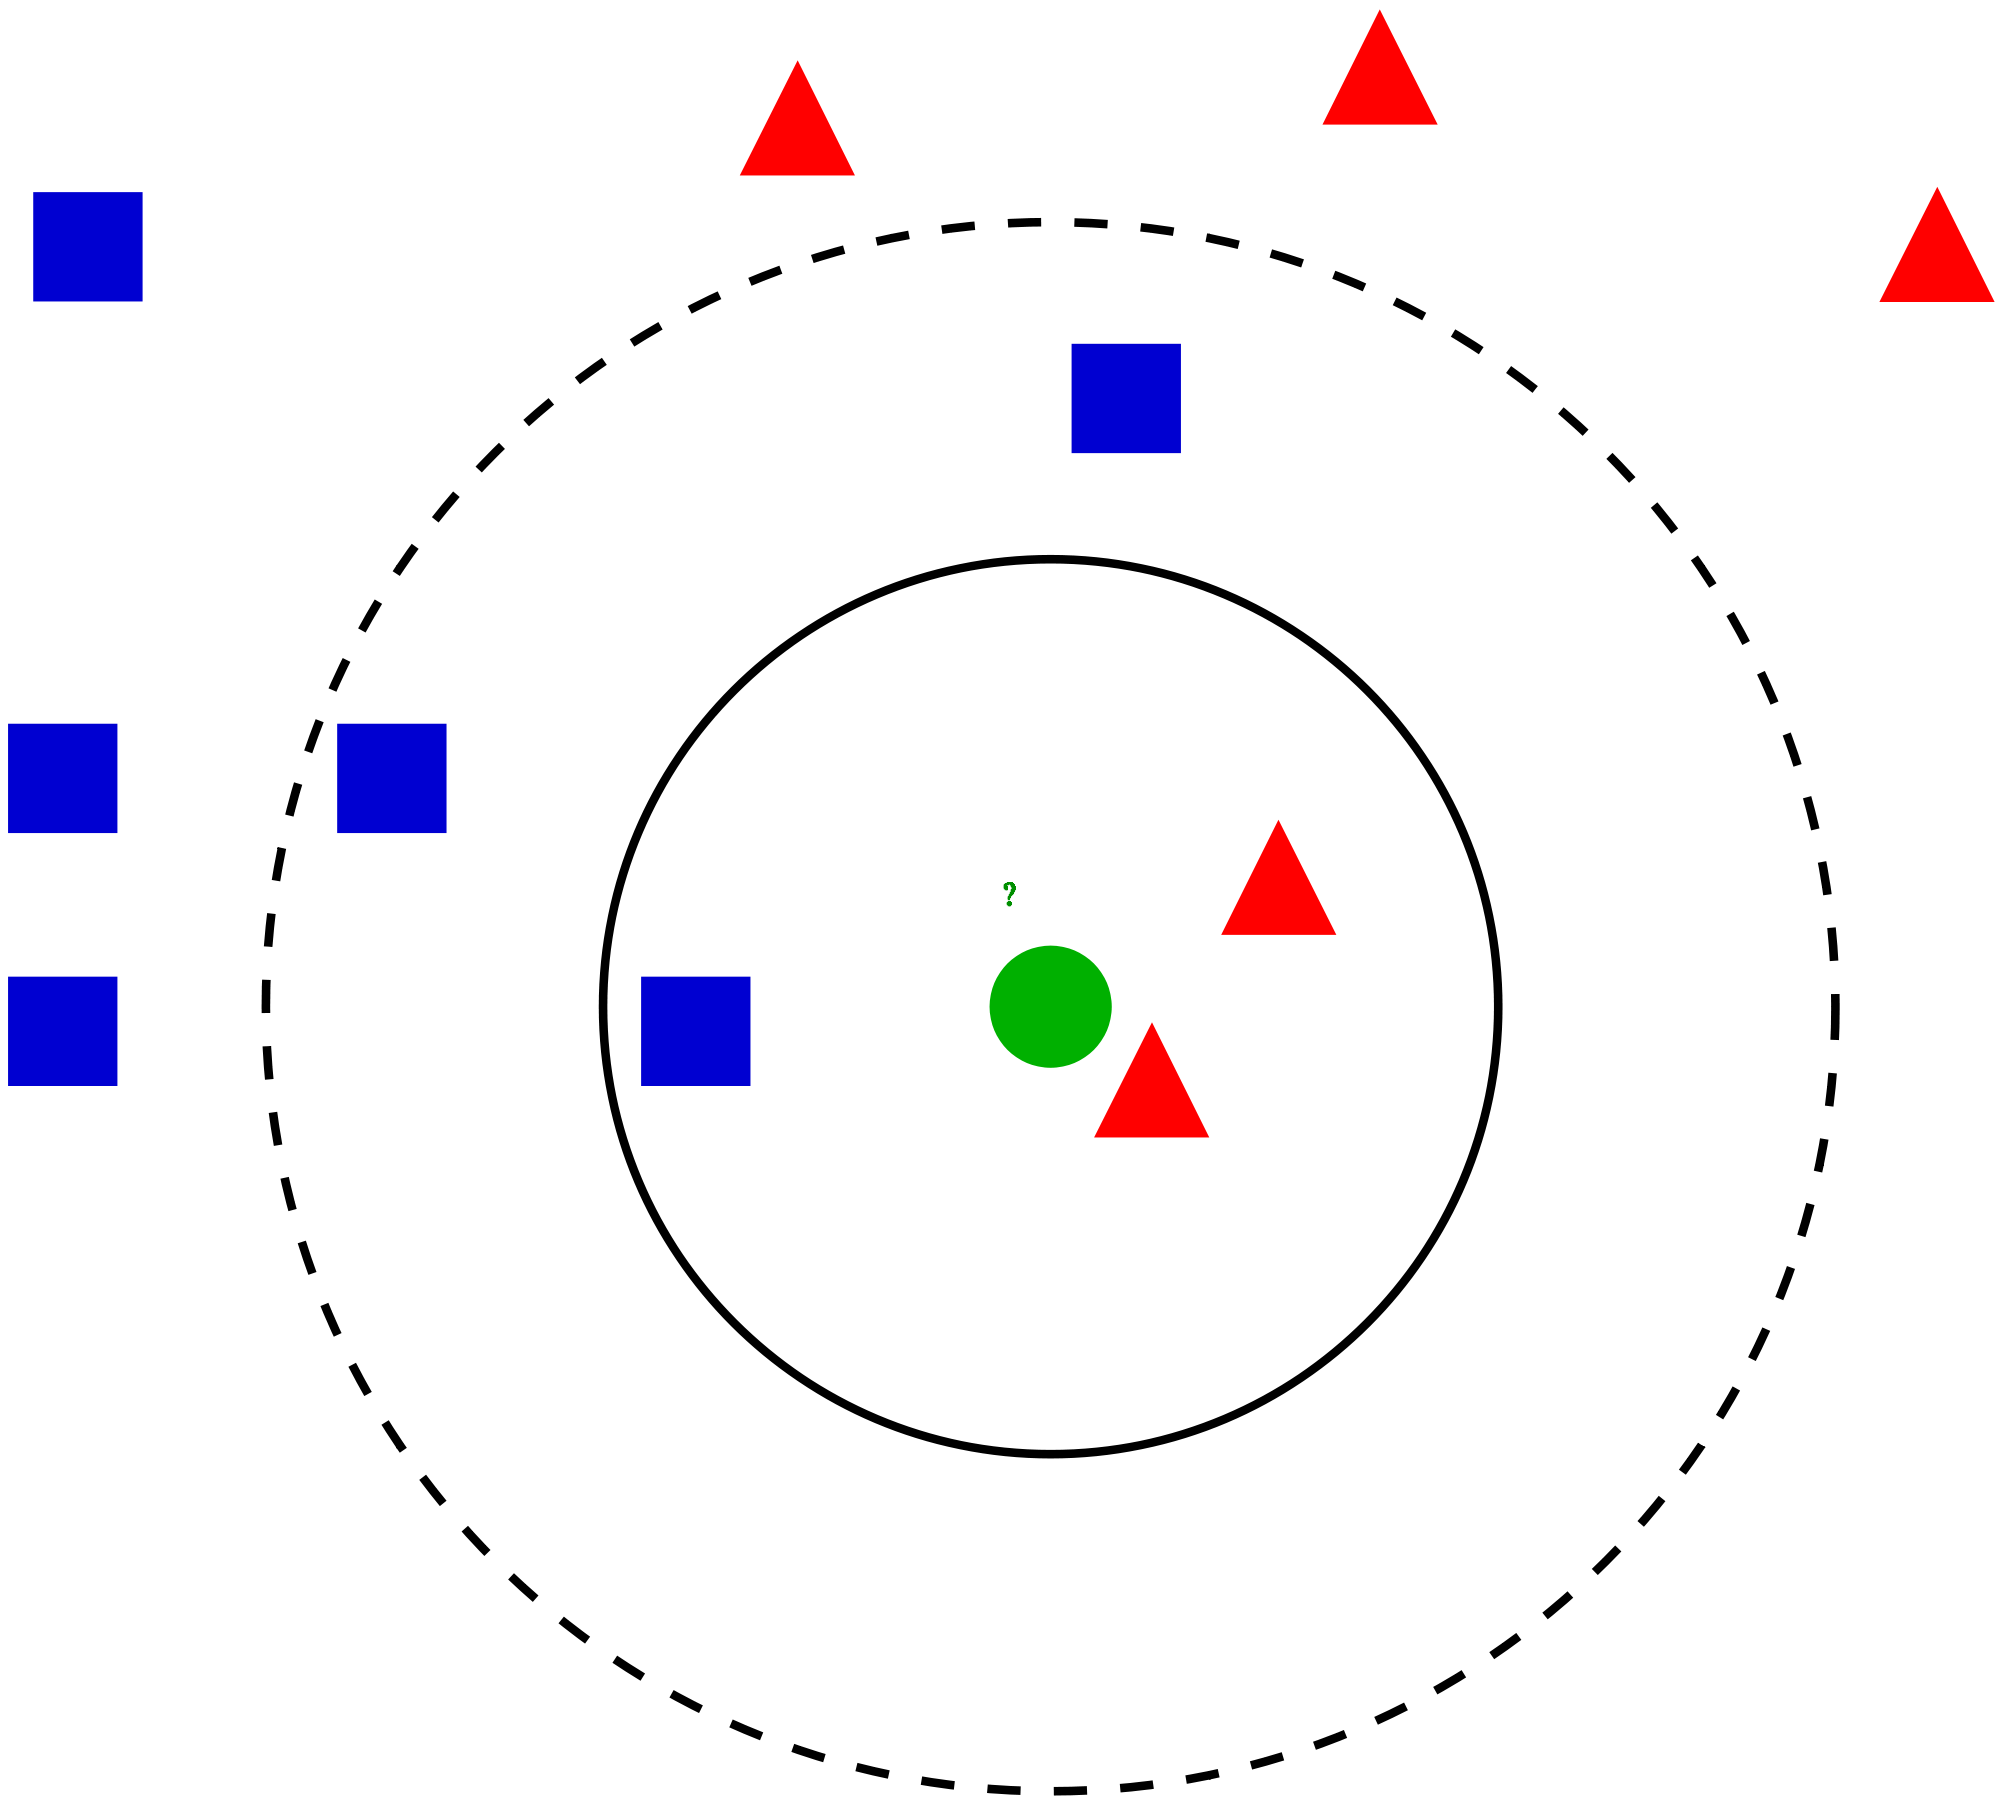
\includegraphics{knn.png}
    \end{center}
\end{frame}

\subsection{Métricas}
\begin{frame}
    \frametitle{Métricas}
    
    
\end{frame}
